
\documentclass[letterpaper, 10 pt, conference]{ieeeconf}  
\IEEEoverridecommandlockouts\overrideIEEEmargins
% See the \addtolength command later in the file to balance the column lengths
% on the last page of the document

\usepackage{graphicx}
\usepackage{amsmath}
\usepackage{tikz}
\usepackage{circuitikz}
\usepackage{calc}
\usepackage{circuitikz}
\usetikzlibrary{calc}
\usepackage{multirow}
\usepackage[document]{ragged2e}

\title{\LARGE \bf
IDE Assignment
}
\vspace{4mm}
\author{Namrath Pinnamaneni \hspace{9cm} August 2022}


\begin{document}
\maketitle

\begin{abstract}
State and Prove Associative Law
\end{abstract}
\tableofcontents

\section{Components}\hfill\break
{
\centering
\begin{tabular}{|c|c|c|}
\hline
$\boldsymbol{Component}$&$\boldsymbol{Value}$&$\boldsymbol{Count}$\\
\hline
Arduino&UNO&1\\
\hline
LED&Red&1\\
\hline
Resistor&220 Ohm&1\\
\hline
Jumper wires&-&as required\\
\hline
\end{tabular}\par
}
\vspace{5mm} %5mm vertical space
\section{Associative Law}
This law states that OR ing or AND ing more than two variables will return the same value irrespective of the grouping of variables in an equation.\\
If a logical operation of any two Boolean variables is performed first and then the same operation is performed with the remaining variable gives the same result, then that logical operation is said to be 'Associative'. The logical OR and logical AND operations of three Boolean variables A, B and C are shown below.
 
\[ A + (B + C) = (A + B) + C  \]
\vspace{1mm} %1mm vertical space
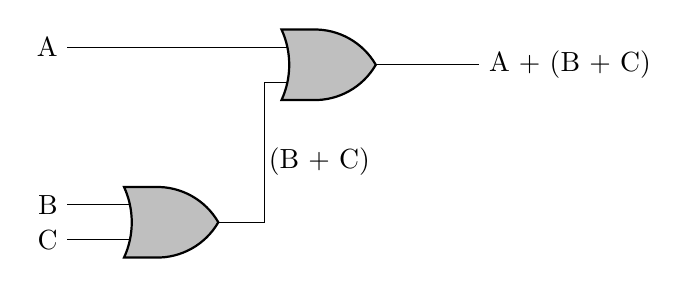
\begin{tikzpicture}
% Circuit style
\ctikzset{
    logic ports=ieee,
    logic ports/scale=0.8,
    logic ports/fill=lightgray
}
% Logic ports
\node[or port] (ORa) at (2,0){};
\node[or port] (ORb) at (0,-2){};
% Connection
\draw (ORa.in 1) -- ++(-2.5,0)node[left](A){A};
\draw (ORb.in 1) -- ++(-0.5,0)node[left](B){B};
\draw (ORb.in 2) -- ++(-0.5,0)node[left](C){C};

\draw (ORb.out) -| (ORa.in 2) ++(0.7,-0.7)node[below]{(B + C)};
\draw (ORa.out) -- ++(1,0) node[right]{A + (B + C) };
\end{tikzpicture}\\
\vspace{5mm} %5mm vertical space
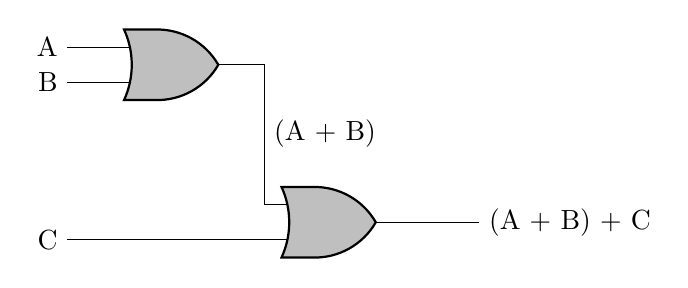
\begin{tikzpicture}
% Circuit style
\ctikzset{
    logic ports=ieee,
    logic ports/scale=0.8,
    logic ports/fill=lightgray
}
% Logic ports
\node[or port] (ORa) at (0,0){};
\node[or port] (ORb) at (2,-2){};
% Connection
\draw (ORa.in 1) -- ++(-0.5,0)node[left](A){A};
\draw (ORa.in 2) -- ++(-0.5,0)node[left](B){B};
\draw (ORb.in 2) -- ++(-2.5,0)node[left](C){C};

\draw (ORa.out) -| (ORb.in 1) ++(0,0.9)node[right]{(A + B)};
\draw (ORb.out) -- ++(1,0) node[right]{(A + B) + C};
\end{tikzpicture}\hfill\break

\[ A . (B . C) = (A . B) . C  \]
\vspace{1mm} %1mm vertical space
% AND Circuits 
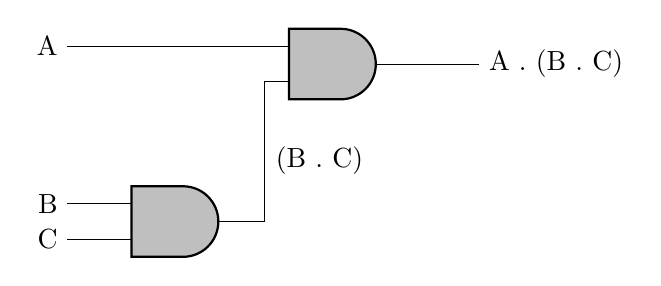
\begin{tikzpicture}
% Circuit style
\ctikzset{
    logic ports=ieee,
    logic ports/scale=0.8,
    logic ports/fill=lightgray
}
% Logic ports
\node[and port] (ANDa) at (3,0){};
\node[and port] (ANDb) at (1,-2){};
% Connection
\draw (ANDa.in 1) -- ++(-2.5,0)node[left](A){A};
\draw (ANDb.in 1) -- ++(-0.5,0)node[left](B){B};
\draw (ANDb.in 2) -- ++(-0.5,0)node[left](C){C};

\draw (ANDb.out) -| (ANDa.in 2) ++(0.7,-0.7)node[below]{(B . C)};
\draw (ANDa.out) -- ++(1,0) node[right]{A . (B . C)};
 
\end{tikzpicture}\\
\vspace{5mm} %5mm vertical space
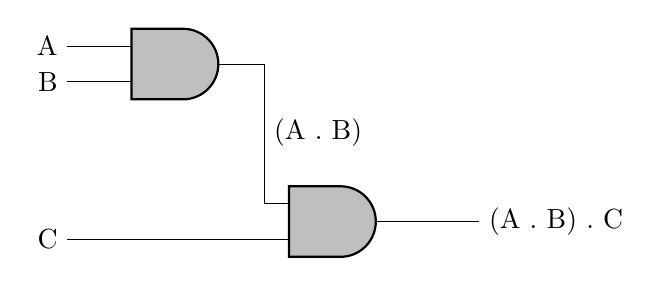
\begin{tikzpicture}
% Circuit style
\ctikzset{
    logic ports=ieee,
    logic ports/scale=0.8,
    logic ports/fill=lightgray
}
% Logic ports
\node[and port] (ANDa) at (0,0){};
\node[and port] (ANDb) at (2,-2){};
% Connection
\draw (ANDa.in 1) -- ++(-0.5,0)node[left](A){A};
\draw (ANDa.in 2) -- ++(-0.5,0)node[left](B){B};
\draw (ANDb.in 2) -- ++(-2.5,0)node[left](C){C};

\draw (ANDa.out) -| (ANDb.in 1) ++(0,0.9)node[right]{(A . B)};
\draw (ANDb.out) -- ++(1,0) node[right]{(A . B) . C};
\end{tikzpicture}\\

\section{Proof}

If A, B and C are three	 variables, then the grouping of 3 variables with 2 variables in each set will be of 3 types, such as (A + B), (B + C) and (C + A).

According to associative law

\[(A + B + C) = (A + B) +C = A + (B + C) = B + (C + A)\]

We know that, \textbf{\textit{A + AB = A}} (according to Absorption law)\\

Now let’s assume that, \[x = A + (B + C)\] and \[y = (A + B) + C\]

According to associative law, we need to prove that \[x = y.\]

Now, find \[Ax = A [ A + (B + C) ]\]

\[ = AA +A (B + C)\]
→ since \(AA = A\)
\[ = A + AB + AC\] 
\[ = (A+ AB) + AC\]
→ since \(A + AB = A\)
\[= A + AC\]
→ since \(A + AC = A\)
\[ = A\]
Therefore \[Ax = A\]
Similarly, for \( Bx = B [ A + (B + C) ]\)
\[ = AB +B (B + C)\]
\[ = AB + BB + BC\]
→ since \(BB = B\)
\[ = AB + B + BC\]
\[ =(B+ BC) + AB\]
→ since \(B + BC = B\)
\[= B + AB\] 
→ since \(B + AB = B\)
\[= B\] 

Using these above equations, we can say that the relation between A, B, C and + operator does not change when multiplied by other variable like x,\\such as \textbf{\textit{xy = yx = x = y}}

\[ yx = ((A + B) + C) x\]
\[ = (A + B) x + Cx\]
\[ = (Ax + Bx) + Cx\]
\[ = (A + B) + C\]
\[ = y xy = (A + (B + C)) y\]
\[ = Ay + (B + C) y\]
\[ = Ay + (By + Cy)\]
\[ = A + (B + C)\]
\[ = x\]

So \textbf{\textit{x = y}}, which means
\[A + (B + C) = (A + B) + C = B + (A + C)\]

\textbf{Example:}

Take three variables 0, 1 and 0, then

According to associative law,
\[(0 + 1) + 0 = 0 + (1 + 0)\]
\[1 + 0 = 0 + 1\]
\[1 = 1\]

Hence associative law is verified.

Hence the Associative law is proved, 
\[(A + B + C) = (A + B) +C = A + (B + C) = B + (C + A)\]

\subsection*{\normalsize Truth Table}
{
\[ A + (B + C) = (A + B) + C  \]
\centering
\begin{tabular}{|c|c|c|c|c|c|c|}
\hline
${A}$&${B}$&${C}$&${(B+C)}$&${A+(B+C)}$&${(A+B)}$&${(A+B)+C}$\\
\hline
0&0&0&0&0&0&0\\%
\hline
0&0&1&1&1&0&1\\%
\hline
0&1&0&1&1&1&1\\%
\hline
0&1&1&1&1&1&1\\%
\hline
1&0&0&0&1&1&1\\%
\hline
1&0&1&1&1&1&1\\%
\hline
1&1&0&1&1&1&1\\%
\hline
1&1&1&1&1&1&1\\%
\hline
\end{tabular}\par
}
\vspace{5mm} %5mm vertical space
\[ A . (B . C) = (A . B) . C  \]
{
\centering
\begin{tabular}{|c|c|c|c|c|c|c|}
\hline
${A}$&${B}$&${C}$&${(B.C)}$&${A.(B.C)}$&${(A.B)}$&${(A.B).C}$\\
\hline
0&0&0&0&0&0&0\\%
\hline
0&0&1&0&0&0&0\\%
\hline
0&1&0&0&0&0&0\\%
\hline
0&1&1&0&0&1&0\\%
\hline
1&0&0&0&0&0&0\\%
\hline
1&0&1&0&0&0&0\\%
\hline
1&1&0&1&0&0&0\\%
\hline
1&1&1&1&1&1&1\\%
\hline
\end{tabular}\par
}
\vspace{5mm} %5mm vertical space
\section{Hardware}
Make connections between Digital Pin 8 of Arduino with LED in Breadboard.
\vspace{5mm} %5mm vertical space
\section{Software}
LED lights up when LHS = RHS\\
\vspace{1mm} %5mm vertical space
Make the connections and connect the arduino to the PC via USB and use below commands
\begin{enumerate}
\item svn co https://github.com/namwave/fwc/ide/assignment
\item cd ide\_assignment
\item pio run
\item pio run \--t upload

\end{enumerate}
\begin{figure}[ht]
\centering
\includegraphics[width=5.2cm, height=7.5cm, angle=90]{result.jpg}
\caption{Result}
\label{fig:result_picture}
\end{figure}


\addtolength{\textheight}{-12cm}   % This command serves to balance the column lengths
                                  % on the last page of the document manually. It shortens
                                  % the textheight of the last page by a suitable amount.
                                  % This command does not take effect until the next page
                                  % so it should come on the page before the last. Make
                                  % sure that you do not shorten the textheight too much.

\end{document}
